%% ------------------------------------------------------------------------- %%
\section{Algoritmos}
\label{sec:algoritmos}

A detecção da \emph{Frequência Fundamental (F0)} ou transcrição melódica é um problema bastante pesquisado e comumente considerado ``resolvido'' no caso de vozes ou instrumentos monofônicos gravados segundo \cite{de2001efficient}.
Porém a questão do tempo real adiciona algumas dificuldades ao problema. Geralmente esses são os requerimentos para os algoritmos em tempo real:

\begin{itemize}
\item Capacidade de funcionar em tempo real
\item Mínimo atraso de saída (latência)
\item Acurácia na presença de ruído
\item Sensibilidade à performance musical
\end{itemize}

Nesse contexto, apresentamos os seguintes algoritmos a serem implementados no \emph{ASyMuT - Automatic System for Music Transcription}:

\begin{itemize}
\item \emph{Harmonic Product Spectrum}
\item \emph{Maximum Likelihood}
\item \emph{Cepstrum-Biased Harmonic Product Spectrum}
\item \emph{Weighted Autocorrelation Function}
\end{itemize}

\subsection{Harmonic Product Spectrum - Espectro do Produto Harmônico}

Esse algoritmo busca por uma frequência cujo produto da magnitude dos primeiros $K$ harmônicos é máximo, calculando a seguinte função para cada frequência: $$Y(\omega) = \prod _{k=1}^{K} \abs{X(\omega k))}$$
E então buscando seu máximo: $$\widehat{Y} = \max\limits_{\omega_i}\{Y(\omega_i)\}$$
Um exemplo pode ser visto na figura \ref{fig:hps2}.

     \begin{figure}%[!htb]
\centering
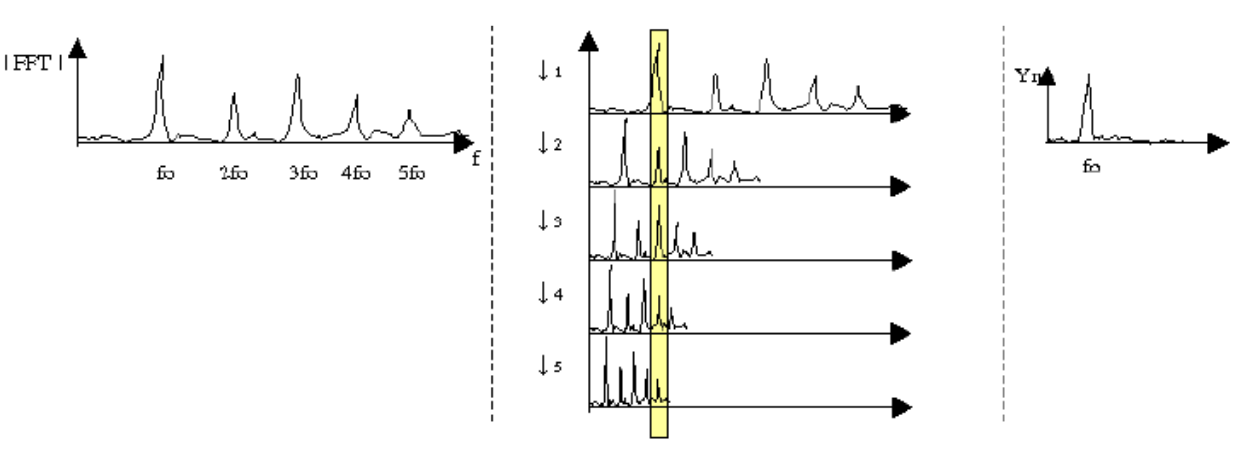
\includegraphics[width=0.85\linewidth]{hps2.png}
\caption{Harmonic Product Spectrum para $K=5$}
\label{fig:hps2}
\end{figure}

\subsection{Maximum Likelihood - Máxima Verossimilhança}

Esse algoritmo busca por um conjunto de possíveis espectros ideais e escolhe aquele que melhor combina com o formato do espectro de entrada. O espectro ideal é definido como um trem de pulsos começando na frequência $\omega$ convoluído com o espectro da janela do sinal e pode ser visto na figura \ref{fig:maxver}.

     \begin{figure}%[!htb]
\centering
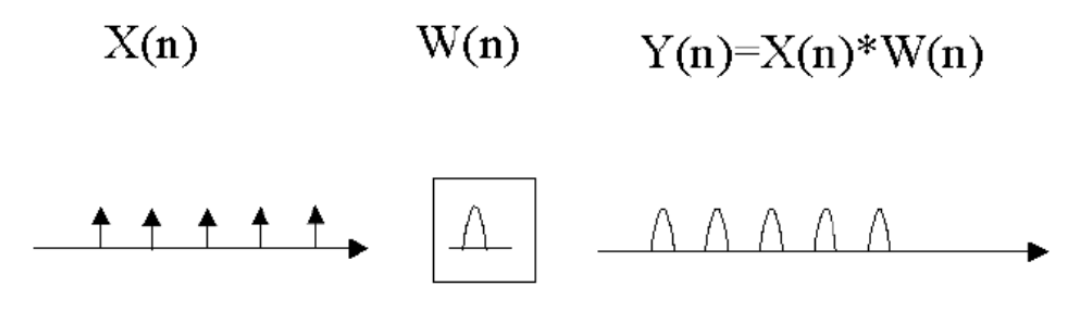
\includegraphics[width=0.6\linewidth]{maxver.png}
\caption{Geração de um espectro ideal.}
\label{fig:maxver}
\end{figure}

Esse processo tenta minimizar o erro entre o espectro da janela e os possíveis espectros candidatos, como ilustrado nas seguintes equações:

$$E(\omega) = \norm{ Y - \tilde{Y}_\omega}^{2}$$

$$= \norm{Y}^{2} + \norm{\tilde{Y}_\omega}^{2} - 2Y\tilde{Y}_\omega^{T}$$


\subsection{Cepstrum-Biased Harmonic Product Spectrum - Espectro do Produto Harmônico basedo no Cepstro}
\subsection{Weighted Autocorrelation Function - Função de autocorrelação ponderada}


%Introduzir os algoritmos que serão melhor explicados no desenvolvimento.
%\begin{itemize}
%\item Explicar os algoritmos utilizados pelo ASyMuT
%\item Dar detalhes da parte matemática dos algoritmos implementados
%\end{itemize}
